\documentclass[12pt,a4paper]{article}
\usepackage[utf8]{inputenc}
\usepackage[T1]{fontenc}
\usepackage[dutch]{babel}
\usepackage{amsmath}
\usepackage{amsfonts}
\usepackage{amssymb}
\usepackage{graphicx}
\usepackage{wrapfig}
\author{Estelle Severs, Matthias Kovacic}
\title{Afleidingen Natuurkunde}
\date{:)}
\begin{document}
	\maketitle
	\tableofcontents
	\newpage
	\section{Algemene afspraken rond dit document}
	\section{Algemene te kennen theorie}
	\subsection{Prefixen}
		\begin{center}
		\begin{tabular}{ | c | c | c | }
		\hline
			 Prefix & Afkorting & Value \\ 
		\hline
			Giga & G & $10^{9}$ \\ 
			Mega & M & $10^{6}$ \\  
 			Kilo & k & $10^{3}$ \\   
 			Hecto & h & $10^{2}$ \\   
 			Deka & da & $10^{1}$ \\   
 			Deci & d & $10^{-1}$ \\   
 			Centi & c & $10^{-2}$ \\   
 			Milli & m & $10^{-3}$ \\   
 			Micro & $\mu$ & $10^{-6}$ \\   
 			Nano & n & $10^{-9}$ \\   
 			Pico & p & $10^{-12}$ \\   
 		\hline
		\end{tabular}
		\end{center}
	\subsection{Vectoren}
	Vergeet niet je vector altijd in componenten te splitsen!
	
	\(A_x = Acos\theta\) en \(A_y = Asin\theta\)
	
	\(A = \sqrt{A_x^2 + A_y^2}\)
	
	\(\theta = tan^{-1}\frac{A_y}{A_x}\)
	\subsubsection{Scalair product}
	De grote van deze vector vermenigvuldigd met de projectie van de andere vector op deze vector. Hieruit krijg je dus een scalar!!
	\[\textbf{A} * \textbf{B} = ABcos\theta\]
	\subsubsection{Vectorproduct}
	Dit product geeft altijd een vector loodrecht op beide vectoren. Deze uitkomst is te vinden met de rechterhandregel. Als je deze nog niet kent: zoekt es op op youtube ;) 
	De grootte is te vinden met volgende formule: 
	\[\textbf{A} x \textbf{B} = ABsin\theta\]
	\newpage
	\section{Deel 1 - Mechanica}
	\section{Kinematica in 1 dimensie}
	2.1-2.6, 2.8-2.9
	\subsection{2.5: Formules bij constante versnelling}
	We nemen aan dat het initiële tijdstip in elk van deze formules altijd 0 is. \((t_{0} = 0)\).
	Vergelijking voor snelheid afleiden: 
	\[\mathbf{a = \frac{dv}{dt} = constante}\]
	$\iff$ \[a dt = dv\]
	$\iff$ \[\int_{v_0}^{v} a \, dt = \int_{0}^{t} \,dv\]
	$\iff$\[v - v_0 = at\]
	$\iff$\[\mathbf{v = v_0 + at}\]
	Vergelijking voor verplaatsing afleiden: 
	\[v = \frac{dx}{dt}\]
	$\iff$\[dx = v dt\]
	$\iff$\[x - x_0 = \int_{0}^{t} v \, dt\]
	$\iff$\[x - x_0 = \int_{0}^{t} (v_0 + at) \, dt\]
	$\iff$\[x - x_0 = \int_{0}^{t} v_0 \, dt + \int_{0}^{t} at \, dt\]
	$\iff$\[\mathbf{x - x_0 = v_0t + a\frac{t^2}{2}}\]
	Alternatieve vergelijking voor snelheid: 
	\[\bar{v} = \frac{v_0 + v}{2} \text{en} t = \frac{v - v_0}{a}\]
	dan geldt voor de vergelijking van verplaatsing: 
	\[x = x_0 + (\frac{v + v_0}{2})(\frac{v - v_0}{a})\]
	$\iff$\[x = x_0 + \frac{v^2 + v_0^2}{2a}\]
	$\iff$\[\mathbf{v^2 = v_0^2 + 2a(x - x_0)}\]
	\section{Kinematica in twee of drie dimensies}
	3.7
	\subsection{Projectiel beweging: formules}
	\begin{figure}[h]
		\centering
		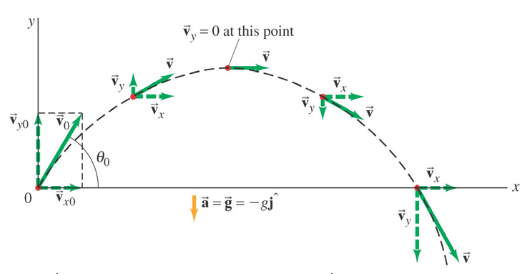
\includegraphics[width=0.7\linewidth]{projectiel}
		\caption{Er zal enkel een in de verticale component een versnelling aanwezig zijn. Hierdoor verandert de snelheid enkel in de verticale component.}
		\label{projectiel}
	\end{figure}
\begin{table}[h]
	\centering
	\begin{tabular}{|c|c|}
		\hline
		\textbf{Horizontaal} & \textbf{Verticaal} \\
		\hline
		\(a_x = 0\)&\(a_y = -g\)  \\
		\hline
		\(v_x(t) = v_{x0}\)&\(v_y(t) = v_{y0} - gt\)  \\
		\hline
		\(x(t) = x_0 + v_{x0}t\)&\(y(t) = y_0 + v_{y0}t - \frac{gt^2}{2}\)  \\
		\hline
	\end{tabular}
\end{table}
	\section{Dynamica: Newton's bewegingswetten}
	4.1-4.7
	\subsection{Eerste wet: inertie}
	Een lichaam in rust (of in eenparige rechtlijnige beweging) zal in rust (eenparige rechtlijnige beweging) blijven tenzij er een uitwendige resulterende kracht inwerkt.
	\[\sum_{i}\overrightarrow{F_i} = 0 \Rightarrow \overrightarrow{a} = 0\]
	\subsection{Tweede wet: versnelling}
	Een grotere kracht op een lichaam met massa m veroorzaakt een grotere versnelling: a \textasciitilde F
	
	Bij een dubbele massa 2m zal eenzelfde kracht slechts een versnelling a/2 veroorzaken: a \textasciitilde 1/m 
	
	\[\sum_{i} \overrightarrow{F_i} = \overrightarrow{F} = m\overrightarrow{a}\]
	\subsection{Derde wet: actie-reactie}
	Bij wisselwerking tussen twee lichamen is de kracht \(\overrightarrow{F_{21}}\) van lichaam 1 op lichaam 2 even groot en tegengesteld aan de kracht \(\overrightarrow{F_{12}}\) van lichaam 2 op lichaam 1.
	\[\overrightarrow{F_{12}} = -\overrightarrow{F_{21}}\]
	Deze krachten komen steeds in paren voor en werken op verschillende voorwerpen.
	\subsection{Gewicht - Gravitatie - Normaalkracht}
	Alle voorwerpen nabij het aardoppervak vallen met dezelfde versnelling $\overrightarrow{g}$. 
	\[\text{Gravitatiekracht: } \overrightarrow{F_G} = m\overrightarrow{g}\]	
	\section{De wetten van Newton: wrijving, cirkelbeweging, weerstandskrachten}
	\subsection{Delen in de Giancoli}
	5.1-5.3, 5.5-5.6
	\section{De zwaartekracht en de synthese van Newton}
	\subsection{Delen in Giancoli}
	6.1-6.4, 6.6
	\section{Arbeid en energie}
	\subsection{Delen in Giancoli}
	7.1, 7.3-7.4 (+14.1)
	\section{Behoud van energie}
	\subsection{Delen in Giancoli}
	8.1-8.3, 8.5, 8.8
	\section{Impuls}
	\subsection{Delen in Giancoli}
	9.1-9.2 (+36.11)
	\section{Rotatie}
	10.1, 10.4, 10.8
	\section{Impulsmoment}
	\subsection{Delen in Giancoli}
	11.3-11.4, 11.6
	\newpage
	
	
	\section{Deel 2 - Elektriciteit}
	\section{Elektrische velden}
	\subsection{Delen in Giancoli}
	21.1-21.2, 21.4-21.11, 21.13 
	\section{De wet van Gauss}
	\subsection{Delen in Giancoli}
	22.1-22.3
	\section{Elektrische potentiaal}
	\subsection{Delen in Giancoli}
	23.1-23.9
	\section{Condensatoren en diëlektrica}
	\subsection{Delen in Giancoli}
	24.2-24.6
	\section{Elektrische stroom en weerstand}
	\subsection{Delen in Giancoli}
	25.1-25.6, 25.8-25.9 (+40.7-40.10)
	\section{Gelijkstroomschakelingen}
	\subsection{Delen in Giancoli}
	26.2-26.5, 26.7
	\newpage
	\section{Deel 3 - Magnetisme}
	Dit is geen deel van het vak in het eerste jaar, maar zal je misschien van pas komen in het tweede jaar ;).
\end{document}